
% Kelas D4 TI 3B Kelompok 3 tugas ke-3
% Diana Satima Gistivani 1154018
% M. Amran Hakim Siregar 1154106
% Indah Rahmawati 1154070
% Rizky Abdul Ghani Suherli 1154058
% Ajrina Darman 1154079

\section{XML Processing} 
\hspace*{0.5in} XML adalah bahasa open source portable yang mungkinkan pemrogram mengemangkan aplikasi yang dapat dibaca oleh aplikasi lain, terlepas dari sistem operasi dan bahasa pengembangnya. 
\vspace{12pt}
 
\hspace*{0.5in} Extensible Markup Languange (XML) adalah bahasa markup seperti HTML atau SGML. Ini direkomendasikan oleh World Wide Web Consortium dan tersedia sebagai standar terbuka. XML sangat berguna untuk mencatat data berukuran kecil dan menengah tanpa memerlukan tulang punggung berbasis SQL. 

\vspace{12pt}
\subsection{Arsitektur Parsing XML dan API} 
 
\hspace*{0.5in} Perpustakaan standar Python menyediakan seperangkat antarmuka minimal tapi berguna untuk bekerja dengan XML.  
 
\hspace*{0.5in} Dua API yang paling dasar dan umum digunakan untuk data XML adalah antarmuka SAX dan DOM. 
 
\hspace*{0.5in} API sederhana untuk XML (SAX): mendaftarkan panggilan kemali untuk acara yang diminati dan kemudian membiarkan parser berjalan melalui dokumen. Ini berguna bila dokumen berukuran besar atau memiliki keterbatasan memori, ini memparsing file tidak pernah tersimpan dalam memori. 
 
\hspace*{0.5in} API Document Objek Model (DOM): ini adalah rekomendasi World Wide Web Consortium dimana keseluruhan file dibaca ke memori dan disimpan dalam bentuk hierarkies (tree-based) untuk mewakili semua fitur dokumen XML.  
 
\hspace*{0.5in} SAX jelas tidak bisa memproses informasi secepat DOM saat bisa bekerjadengan file besar. Di sisi lain, menggunakan DOM secara eklusifenar-benar dapat membunuh sumber daya, terutama jika digunakan pada banyak file kecil. 
 
\hspace*{0.5in} SAX hanya bisa dibaca sementara DOM mengizinkan perubahan pada file XML. Kedua API yang berbeda ini saling melengkapi satu sama lain, tidak ada alasan mengapa tidak dapat menggunakannya untuk proyek besar. 
\vspace{12pt}
 
Contoh: 
\begin{verbatim} 
<collection shelf="New Arrivals"> 
 
<movie title="Enemy Behind"> 
 
    <type>War, Thriller</type> 
 
    <format>DVD</format> 
 
    <year>2003</year> 
 
    <rating>PG</rating> 
 
    <stars>10</stars> 
 
    <description>Talk about a US-Japan war</description> 
 
</movie> 
 
<movie title="Transformers"> 
 
    <type>Anime, Science Fiction</type> 
 
    <format>DVD</format> 
 
    <year>1989</year> 
 
    <rating>R</rating> 
 
    <stars>8</stars> 
 
    <description>A schientific fiction</description> 
 
</movie> 
 
    <movie title="Trigun"> 
 
    <type>Anime, Action</type> 
 
    <format>DVD</format> 
 
    <episodes>4</episodes> 
 
    <rating>PG</rating> 
 
    <stars>10</stars> 
 
    <description>Vash the Stampede!</description> 
 
</movie> 
 
<movie title="Ishtar"> 
 
   <type>Comedy</type> 
 
   <format>VHS</format> 
 
   <rating>PG</rating> 
 
   <stars>2</stars> 
 
   <description>Viewable boredom</description> 
 
</movie> 
</collection>
\end{verbatim}
 
\vspace{10pt}
\subsection{Parsing XML dengan API SAX} 
 
\hspace*{0.5in} SAX adalah antarmuka standar untuk parsing XML berbasis event. Parsing XML dengan SAX umumnya mengharuskan untuk membuat C\textit{ontrolHandler }dengan subclassing xml.sax \textit{controlhandler}. 
 
\hspace*{0.5in} \textit{ControlHandler }menangani tag dan atribut tertentu dari XML. Objek \textit{ControlHandler }menyediakan metode untuk menangani berbagai aktivitas parsing. Parsing memanggil metode \textit{ControlHandler }saat memparsing file XML. 

\hspace*{0.5in} Metode \textit{startDocument} dan \textit{endDocument} disebut awal dan akhir setiap elemen. Jika parsing tidak dalam mode namespace, metode \textit{startElement} (tag attribute) dan \textit{endElement} (tag) dipanggil. Jika tidak, metode yang sesuai \textit{startElemenNS} dan \textit{endElemenNS} dipanggil. Disini, tah adalah tag elemen dan atribut adalah atribut.  
 
\hspace*{0.5in} Metode-metode berikut membuat objek parsing baru dan mengembalikannya. Objek parsing diuat akan menjadi tipe parsing pertama yang ditemukan sistem.  
{\fontsize{10pt}{10pt}\selectfont xml.sax.make $  \_  $parser([parser $  \_  $list])} .Parameter 
Parser $  \_  $list pilihan argumen yang terdiri dari daftar parsing untuk digunakan yang semuanya harus menerapkan metode \textit{make $  \_  $parse} 
 
\hspace*{0.5in} Metode-metode berikut membuat parsing SAX dan menggunakannya untuk mengurai dokumen {\fontsize{10pt}{10pt}\selectfont xml.sax.parser(xmlfile, contenthandler[, errorhandler])}. Berikut adalah detail dari parameternya: 
 
\begin{itemize}
\item \textit{Xmlfile } 

Ini adalah nama file XML yang bisa dibaca. 
\item \textit{ContentHandler } 

Ini harus menjadi objek \textit{ContenHandler} 
\item \textit{ErrorHandler} 

Jika ditentukan, e\textit{rrorhandler} harus menjadi objek \textit{ErrorHandler} SAX 
\item Metode\textit{ parseString}
\end{itemize}

\vspace{12pt} 
Membuat parsing SAX dan mengurai string XML yang ditentukan : 
{\fontsize{10pt}{10pt}\selectfont xml.sax.parsertring(xmlstring,contenthandler[, errorhandler])}.
 
\vspace{12pt}
Brikut ini adalah detail nama dar parameter : 
\begin{itemize}
\item {XMLstring} 

Nama dari string yang bisa dibaca 
 
\item {ContentHandler} 

Menjadi objek ContenHandler 
 
\item {ErrorHandler} 

Menjadi objek ErorHandler SAX 
\end{itemize}

\vspace{12pt}
Contoh : 
\begin{verbatim}
 $  \#  $!/usr/bin/python 
 
import xml.sax 
 
class MovieHandler( xml.sax.ContentHandler ): 
 
    def  $  \_  $ $  \_  $init $  \_  $ $  \_  $(self): 
 
      self.CurrentData = "" 
 
      self.type = "" 
 
      self.format = "" 
 
      self.year = "" 
 
      self.rating = "" 
 
      self.stars = "" 
 
     self.description = "" 
 
   $  \#  $ Call when an element starts 
 
   def startElement(self, tag, attributes): 
 
     self.CurrentData = tag 
 
     if tag == "movie": 
 
     print "*****Movie*****" 
 
     title = attributes["title"] 
 
     print "Title:", title 
 
   $  \#  $ Call when an elements ends 
 
  def endElement(self, tag): 
 
     if self.CurrentData == "type": 
 
     print "Type:", self.type 
 
     elif self.CurrentData == "format": 
 
     print "Format:", self.format 
 
     elif self.CurrentData == "year": 
 
     print "Year:", self.year 
 
     elif self.CurrentData == "rating": 
 
     print "Rating:", self.rating 
 
    elif self.CurrentData == "stars": 
 
    print "Stars:", self.stars 
 
    elif self.CurrentData == "description": 
 
    print "Description:", self.description 
 
    self.CurrentData = "" 

    $  \#  $ Call when a character is read 
 
    def characters(self, content): 
 
    if self.CurrentData == "type": 
 
    self.type = content 
 
    elif self.CurrentData == "format": 
 
    self.format = content 
 
    elif self.CurrentData == "year": 
 
    self.year = content 
 
    elif self.CurrentData == "rating": 
 
    self.rating = content 
 
    elif self.CurrentData == "stars": 
 
    self.stars = content 
 
    elif self.CurrentData == "description": 
 
    self.description = content 
 
 
if (  $  \_  $ $  \_  $name $  \_  $ $  \_  $ == " $ 
\_  $ $  \_  $main $  \_  $ $  \_  $"): 
 
    $  \#  $ create an XMLReader 
 
    parser = xml.sax.make $  \_  $parser() 
 
    $  \#  $ turn off namepsaces 
 
    parser.setFeature(xml.sax.handler.feature $  \_  
    $namespaces, 0) 

   $  \#  $ override the default ContextHandler 
 
   Handler = MovieHandler() 
 
   parser.setContentHandler( Handler )   
 
   parser.parse("movies.xml") 
\end{verbatim}
\vspace{12pt}
 
Ini akan menghasilkan hasil sebagai berikut: 
 
{\fontsize{10pt}{10pt}\selectfont *****Movie******} 
 
{\fontsize{10pt}{10pt}\selectfont *****Movie*****} 
 
{\fontsize{10pt}{10pt}\selectfont Title: Enemy Behind} 
 
{\fontsize{10pt}{10pt}\selectfont Type: War, Thriller} 
 
{\fontsize{10pt}{10pt}\selectfont Format: DVD} 
 
{\fontsize{10pt}{10pt}\selectfont Year: 2003} 
 
{\fontsize{10pt}{10pt}\selectfont Rating: PG} 
 
{\fontsize{10pt}{10pt}\selectfont Stars: 10} 
 
{\fontsize{10pt}{10pt}\selectfont Description: Talk about a US-Japan war} 
 
{\fontsize{10pt}{10pt}\selectfont *****Movie*****} 
 
{\fontsize{10pt}{10pt}\selectfont Title: Transformers} 
 
{\fontsize{10pt}{10pt}\selectfont Type: Anime, Science Fiction} 
 
{\fontsize{10pt}{10pt}\selectfont Format: DVD} 
 
{\fontsize{10pt}{10pt}\selectfont Year: 1989} 
 
{\fontsize{10pt}{10pt}\selectfont Rating: R} 
 
{\fontsize{10pt}{10pt}\selectfont Stars: 8} 
 
{\fontsize{10pt}{10pt}\selectfont Description: A schientific fiction} 
 
{\fontsize{10pt}{10pt}\selectfont *****Movie*****} 
 
{\fontsize{10pt}{10pt}\selectfont Title: Trigun} 
 
{\fontsize{10pt}{10pt}\selectfont Type: Anime, Action} 
 
{\fontsize{10pt}{10pt}\selectfont Format: DVD} 
 
{\fontsize{10pt}{10pt}\selectfont Rating: PG} 
 
{\fontsize{10pt}{10pt}\selectfont Stars: 10} 
 
{\fontsize{10pt}{10pt}\selectfont Description: Vash the Stampede!} 
 
{\fontsize{10pt}{10pt}\selectfont *****Movie*****} 
 
{\fontsize{10pt}{10pt}\selectfont Title: Ishtar} 
 
{\fontsize{10pt}{10pt}\selectfont Type: Comedy} 
 
{\fontsize{10pt}{10pt}\selectfont Format: VHS} 
 
{\fontsize{10pt}{10pt}\selectfont Rating: PG} 
 
{\fontsize{10pt}{10pt}\selectfont Stars: 2} 
 
\vspace{10pt}
 
\subsection{Parsing XML dengan API DOM} 
 
\hspace*{0.5in} Document Ovject Model (DOM) adalah API lintas bahasa dari World Wide Web Consortium (W3C) untuk mengakses dan memodifikasi dokumen XML. 
 
\hspace*{0.5in} DOM sangat berguna untuk aplikasi akses acak. SAX hanya memungkinkan melihat satu bit dokumen sekaligus. Jika melihat satu elemen SAX, tidak memiliki akses ke yang lain. 
 
\hspace*{0.5in} Berikut adalah cara termudah untuk memuat dokumen XML dengan cepat dan membuat objek minidom menggunakan modul xml.dom. Objek minidom menyediakan metode parsing sederhana yang dengan cepat memuat pohon DOM dari file XML. 
 
\hspace*{0.5in} Contoh~frase memanggil fungsi  parsing (file [,parsing]) dari objek minidokumen untuk mengurai file XML yang ditunjuk oleh file ke objek pohon DOM. 

contoh:
\begin{verbatim} 
 $  \#  $!/usr/bin/python 
 
from xml.dom.minidom import parse 
 
import xml.dom.minidom 
 
 $  \#  $ Open XML document using minidom parser 
 
DOMTree = xml.dom.minidom.parse("movies.xml") 
 
collection = DOMTree.documentElement 
 
if collection.hasAttribute("shelf"): 
 
   print "Root element :  $  \%  $s"  $  \%  $ collection.
   getAttribute("shelf") 
 
 $  \#  $ Get all the movies in the collection 
 
movies = collection.getElementsByTagName("movie") 
 
 $  \#  $ Print detail of each movie. 
 
for movie in movies: 
 
   print "*****Movie*****" 
 
   if movie.hasAttribute("title"): 
 
   print "Title:  $  \%  $s"  $  \%  $ movie.getAttribute
   ("title") 

   type = movie.getElementsByTagName('type')[0] 
 
   print "Type:  $  \%  $s"  $  \%  $ type.childNodes
   [0].data 
 
   format = movie.getElementsByTagName('format')[0] 
 
   print "Format:  $  \%  $s"  $  \%  $ format.childNodes
   [0].data 
 
   rating = movie.getElementsByTagName('rating')[0] 
 
   print "Rating:  $  \%  $s"  $  \%  $ rating.childNodes
   [0].data 
 
   description = movie.getElementsByTagName('description')
   [0] 
 
   print "Description:  $  \%  $s"  $  \%  $ description.
   childNodes[0].data 
\end{verbatim}

\vspace{12pt}
Ini akan menghasilkan hasil sebagai berikut : 
 
Root element : New Arrivals 
 
*****Movie***** 
 
Title: Enemy Behind 
 
Type: War, Thriller 
 
Format: DVD 
 
Rating: PG 
 
Description: Talk about a US-Japan war 
 
*****Movie***** 
 
Title: Transformers 
 
Type: Anime, Science Fiction 
 
Format: DVD 
 
Rating: R 
 
Description: A schientific fiction 
 
*****Movie***** 
 
Title: Trigun 
 
Type: Anime, Action 
 
Format: DVD 
 
Rating: PG 
 
Description: Vash the Stampede! 
 
*****Movie***** 
 
Title: Ishtar 
 
Type: Comedy 
 
Format: VHS 
 
Rating: PG 
 
Description: Viewable boredom 
\vspace{10pt}
 
\subsection{ Membangun Parsing Document XML menggunakan Python} 
 
\hspace*{0.5in} Python mendukung untuk bekerja dengan berbagai bentuk markup data terstruktur. Selain mengurai xml.etree. \textit{ElementTree} mendukung pembuatan dokumen XML yang terbentuk dengan baik dari objek elemen yang dibangun dalam aplikasi. Kelas elemen digunakakan saat sebuah dokumen diurai untuk mengetahui bagaimana menghasilkan bentuk serial dari isinya kemudian dapat ditulis ke sebuah file.  
 
\hspace*{0.5in} Untuk membuat instance elemeb gunakan fungsi elemen contructor dan \textit{SubElemen()} pabrik. 
contoh :
\begin{verbatim}
Import xml.etree.ElementTree as xml 

     filename =  $ " $/home/abc/Desktop/test $  \_  $xml
     .xml $ " $} 
 
     toot = xml.Element( $ " $Users $ " $)} 
 
     userelement = xml.Element( $ " $user $ " $)} 
 
     root.append(userelement)} 
\end{verbatim}

\vspace{10pt}
Bila menjalankan ini, akan menghasilkan sebagai berikut : 
 
{\fontsize{10pt}{10pt}\selectfont <Users>} 
 
{\fontsize{10pt}{10pt}\selectfont  \hspace*{0.5in} <user>} 
 
{\fontsize{10pt}{10pt}\selectfont  \hspace*{0.5in} <user>} 
 
{\fontsize{10pt}{10pt}\selectfont </Users>} 


\vspace{50pt} 
Tambahkan anak-anak pegguna :
\begin{verbatim} 
Uid = xml.SubElement(userelement,  $ " $uid $ " $)} 
 
Uid.text =  $ " $1 $ " $} 
 
FirstName = xml.SubElement(userelement,  $ " $FirstName 
$ " $)} 
 
FirstName.text =  $ " $testuser $ " $} 
 
LastName = xml.SubElement(userelement,  $ " $LastName
$ " $} 
 
LastName.text =  $ " $testuser $ " $} 
 
Email = xml.SubElement(userelement,  $ " $Email $ " $)} 
 
Email.text = {mailto:testuser@test.com}{testuser@test.com}
} 
 
state = xml.SubElement(userelemet,  $ " $state $ " $)} 
 
state.text =  $ " $xyz $ " $} 
 
location = xml.SubElement(userelement,  $ " $location)} 
 
location.text = abc} 
 
tree = xml.ElementTree(root)} 
 
with open(filename,  $ " $w $ " $) as fh:} 
 
tree.write(fh)} 
\end{verbatim}

\vspace{12pt}
\hspace*{0.5in} Pertama buat elemen root dengan mengunakan fungsi \textit{ElementTree}. Kemudian membuat elemen pegguna dan menambahkannya ke root. Selanjutnya membuat \textit{SubElement }dengan melewatkan elemen pengguna (userelement) ke \textit{SubElemen} beserta namanya seperto  $ " $FirstName $ " $. Kemudian untuk setiap \textit{SubElement} tetapkan properti teks untuk memberi nilai. Di akhir, membuat \textit{ElementTree} dan menggunakannya untuk menulis XML ke file.  Jika menjalankan ini akan menjadi sebagai berikut : 
 
 {\fontsize{10pt}{10pt}\selectfont <users>} 
 
{\fontsize{10pt}{10pt}\selectfont  \hspace*{0.5in} <user>} 
 
{\fontsize{10pt}{10pt}\selectfont  \hspace*{0.5in}  \hspace*{0.5in} <uid>1</uid>} 
 
{\fontsize{10pt}{10pt}\selectfont  \hspace*{0.5in}  \hspace*{0.5in} <FirstName>testuser</FirstName>} 
 
{\fontsize{10pt}{10pt}\selectfont  \hspace*{0.5in}  \hspace*{0.5in} <LastName>testuser</LastName>} 
 
{\fontsize{10pt}{10pt}\selectfont  \hspace*{0.5in}  \hspace*{0.5in} <state>xyz</state>} 
 
{\fontsize{10pt}{10pt}\selectfont  \hspace*{0.5in}  \hspace*{0.5in} <location>abc</location>} 
 
{\fontsize{10pt}{10pt}\selectfont  \hspace*{0.5in} </user>} 
 
{\fontsize{10pt}{10pt}\selectfont </Users>} 
\vspace{10pt}
 
Parsing XML Documen : 
\begin{verbatim} 
import xml.etree.ElementTree as ET} 
 
tree = ET.parse(‘Your $  \_  $XML $  \_  $file $  \_  
$path’)} 
 
 root = tree.getroot()} 
\end{verbatim}

\section{Kerentanan XML}
\hspace*{0.5in} Modul pemrosesan XML tidak aman terhadap data yang dibuat. Penyerang dapat menyalahgunakan kerentanan untuk penolakan serangan layanan, mengakses file lokal, menghasilkan koneksi jaringan ke mesin lain, atau menghindari firewall. Serangan terhadap penyalahgunaan XML fitur asing seperti inline DTD (document type definition) dengan entitas. Tabel berikut memberikan gambaran umum tentang serangan yang diketahui dan jika berbagai modul rentan terhadapnya :


\begin{table}[ht]
	\caption{Ukuran}
	\begin{tabular*}{\textwidth}{@{\extracolsep{\fill}}lcc}
		\hline
		Kind&  Sax&\cr
		\hline
		billion laughs&Vulnerable\cr
		quadratic blowup&Vulnerable\cr
		external entity expansion&Vulnerable&\cr
		DTD retrieval&Vulnerable&\cr
		decompression bomb&Safe\cr
		\hline
	\end{tabular*}
	\begin{tablenotes}
	\end{tablenotes}
\end{table}

\section{Python XML Processing}
  XML adalah bahasa open source portable yang mungkinkan pemrogram mengemangkan aplikasi yang dapat dibaca oleh aplikasi lain, bahasa markup untuk keperluan umum yang disarankan oleh W3C untuk membuat dokumen markup keperluan pertukaran data antar sistem yang beraneka ragam. XML merupakan kelanjutan dari HTML (HyperText Markup Language) yang merupakan bahasa standar untuk melacak Internet.
terlepas dari sistem operasi dan bahasa pengembangnya .
\subsection{Apa itu XML}
  Extensible Markup Languange (XML) adalah bahasa markup seperti HTML atau SGML. 
Ini direkomendasikan oleh World Wide Web Consortium dan tersedia sebagai standar terbuka.
XML sangat berguna untuk mencatat data berukuran kecil dan menengah tanpa memerlukan tulang punggung berbasis SQL  
Pada kenyataanya dalam dunia komputer, sistem komputer dan database mengandung data yang tidak kompatibel satu sama lain. Dengan demikian tidak mungkin terjadinya pertukaran data melalui internet jika terdapat perbedaan sistem operasi dan aplikasi database yang digunakan.
Dengan menggunakan XML untuk pertukaran data, masalah perbedaan platform dan aplikasi tidak perlu diresahkan lagi. karena data yang disimpan pada XML dapat dibaca oleh berbagai macam platform dan aplikasi.

\subsection{Keunggulan dan Kelemahan Python XML Processing}
\subsubsection{Keunggulan Python XML Processing}
Keunggulan dari python dapat dijabarkan dari faktor-faktor berikut ini :

\begin{enumerate}
\item Quality : Python merupakan piranti lunak yang memakai meodologi reusability sehingga komponen-komponen pembangun piranti      lunak mudah digunakan dan diatur.
\item Productivity : penulisan program menggunakan python lebih mudah, karena interpreter menangani source code secara terpisah pada lower-level language.Interpreter menangani tipe deklarasi variabel,manajemen memory dan source code.
\item Portability : program python dapat dieksekusi di berbagai jenis komputer.Dengan demikian proses eksekusi program dapat dilakukan tanpa mengubah source code program.
\item Integration : phyton dirancang untuk dapat berinteraksi dengan aplikasi lain.Dengan demikian,program yang dibangun dengan bahasa pemrograman lain dapat dieksekusi dengan mudah padascript phyton dengan menggunakan function bahasa pemrograman lainnya.
\item Tidak ada tahapan kompilasi dan penyambungan (link) sehingga kecepatan perubahan pada masa pembuatan sistem aplikasi meningkat.
\item Tidak ada deklarasi tipe data yang merumitkan sehingga program menjadi lebih sederhana, singkat, dan fleksible.
\item Manajemen memori otomatis yaitu kumpulan sampah memori sehingga dapat menghindari pencacatan kode.
\item Tipe data dan operasi tingkat tinggi yaitu kecepatan pembuatan sistem aplikasi menggunakan tipe objek yang telah ada.
\item Pemrograman berorientasi objek.
\item Pelekatan dan perluasan dalam C.
\item Terdapat kelas, modul, eksepsi sehingga terdapat dukungan pemrograman skala besar secara modular.
\item Pemuatan dinamis modul C sehingga ekstensi menjadi sederhana dan berkas biner yang kecil
\item Pemuatan kembali secara dinamis modul phyton seperti memodifikasi aplikasi tanpa menghentikannya.
\item Model objek universal kelas Satu.
\item Konstruksi pada saat aplikasi berjalan.
\item Interaktif, dinamis dan alamiah.
\item Akses hingga informasi interpreter.
\item Portabilitas secara luas seperti pemrograman antar platform tanpa ports.
\item Kompilasi untuk portable kode byte sehingga kecepatan eksekusi bertambah dan melindungi kode sumber.
\item Antarmuka terpasang untuk pelayanan keluar seperti perangkat Bantu system, GUI, persistence, database, dll.
\item Mudah pemeliharaannya.
\item Sederhana. xml lebih sederhana.
\item Mudah dipindah-pindahkan (Portability). XML mempunyai kemudahan perbindahan (portabilitas) yang lebih bagus.
\item Intelligence. XML dapat menangani beberapa tingkat (level) kompleksitas.
\item Dapat beradaptasi. dapat mengadaptasi untuk membuat bahasa sendiri. Seperti microsoft membuat bahasa MSXML atau macromedia mengembangkan MXML.
\end{enumerate}
 
\subsection {Arsitektur XML dan API}
  Perpustakaan standar Python menyediakan seperangkat antarmuka minimal tapi berguna untuk bekerja dengan XML. Dua API yang paling dasar dan umum digunakan untuk data XML adalah antarmuka SAX dan DOM. 
\subsubsection {System Arsitektur XML}
Sistem terdiri dari 3 lapisan yaitu :
\begin{enumerate}
\item lapisan database :Lapisan ini digunakan untuk menyimpan dokumen XML.Dalam system ini digunakan DBMS SQL Server.SQL
Server mengenalkan tipe data XML.Tipe data ini dapat digunakan dalam definisi tabel untuk mendefinisikan tipe sebuah kolom, tipe variabel dalam kode prosedural Transact-SQL, dan sebagai parameter prosedur.
\item lapisan bahasa query : XML, seperti basisdata relasional, mempunyai bahasa query sendiri yang dioptimasi untuk format data.Berpasangan dengan tipe data xml, hal ini mempercepat dan mengefisienkan penyimpanan dan temukembali data XML.
\item lapisan aplikasi : Lapisan ini merupakan antarmuka menggunakan bahasa Indonesia. Bahasa pemrograman yang digunakan adalah Java.Java menyediakan banyak fasilitas yang memudahkan untuk mengimplementasikan system yang dibuat.
\end{enumerate}

\subsection {Kebutuhan Pengguna XML}
\subsubsection {Pengguna XML}
Dari perspektif bisnis hampir semua tipe data bisa direpresentasikan sebagai XML, dengan suatu grammar yang mendeskripsikan strukturnya. terdapat sejumlah lapangan bisnis yang akan mendapatkan keuntungan secara lansung dari pengguna XML, yaitu :
\begin{enumerate}
\item E-commerce.
\item Platform indepedence.
\item Kemampuan pengaksesan data.
\item Penyerdahanaan aplikasi.
\item Memungkinkan sharing data lewat internet.
\end{enumerate}


\subsubsection {SAX}
  SAX adalah singkatan dari Simple API for XML. API sendiri adalah singkatan dari Application Program Interface.Seperti namanya, dibanding DOM Parser, isi program SAX Parser lebih sederhana. SAX parser bekerja berdasarkan apa yang disebut event-based. API sederhana untuk XML (SAX): mendaftarkan panggilan kemali untuk acara yang diminati dan kemudian membiarkan parser berjalan melalui dokumen. Ini berguna bila dokumen berukuran besar atau memiliki keterbatasan memori, ini memparsing file tidak pernah tersimpan dalam memori. Biasanya juga SAX ini dapat di pakai oleh Generator untuk membaca file XML dan pesan SAX ini juga biasa disebut dengan istilah event. SAX akan di kirimkan oleh Generator ke pipeline. SAX atau event ini juga dapat mengirimkan sebuah dokumen atau lampiran yang artinya SAX atau event ini dapat di proses nantinya.
  
\subsubsection {DOM}
  API Document Objek Model (DOM): ini adalah rekomendasi World Wide Web Consortium dimana keseluruhan file dibaca ke memori dan disimpan dalam bentuk hierarkies (tree-based) untuk mewakili semua fitur dokumen XML. DOM merupakan singkatan dari dari Document Object Model.DOM Parser menterjemahkan dokumen XML dan menempatkan elemen-elemen yang ditemuinya ketika memproses dokumen ke dalam struktur pohon.
  DOM memproses struktur dokumen dengan perulangan.empat kondisi yang cocok untuk menggunakan DOM, yaitu:
\begin{enumerate}
\item Ketika terjadi modifikasi sebuah dokumen XML, seperti mengurutkan elemen atau mengubah letak elemen pada suatu pohon elemen satu ke lainnya.
\item Ketika dokumen XML di memori harus dibagi dengan aplikasi lainnya setelah proses parsing.
\item Ketika ukuran dokumen XML tidak terlalu besar.
\item Ketika aplikasi memulai proses utama setelah proses pengesahan.
\end{enumerate}

SAX jelas tidak bisa memproses informasi secepat DOM saat bisa bekerjadengan file besar. Di sisi lain, menggunakan DOM secara eklusifenar-benar dapat membunuh sumber daya, terutama jika digunakan pada banyak file kecil. SAX hanya bisa dibaca sementara DOM mengizinkan perubahan pada file XML. Kedua API yang berbeda ini saling melengkapi satu sama lain, tidak ada alasan mengapa tidak dapat menggunakannya untuk proyek besar. 

Contoh Do: 
\begin{verbatim}
<collection shelf="New Arrivals"> 
<movie title="Enemy Behind"> 
  <type>War, Thriller</type> 
  <format>DVD</format> 
  <year>2003</year> 
  <rating>PG</rating> 
  <stars>10</stars>
  <description>Talk about a US-Japan war</description> 
</movie> 
<movie title="Transformers"> 
  <type>Anime, Science Fiction</type> 
  <format>DVD</format> 
  <year>1989</year> 
  <rating>R</rating> 
  <stars>8</stars> 
  <description>A schientific fiction</description> 
</movie> 
  <movie title="Trigun"> 
  <type>Anime, Action</type> 
  <format>DVD</format> 
  <episodes>4</episodes>  
  <rating>PG</rating> 
  <stars>10</stars> 
  <description>Vash the Stampede!</description> 
</movie>
<movie title="Ishtar"> 
  <type>Comedy</type> 
  <format>VHS</format> 
  <rating>PG</rating> 
  <stars>2</stars> 
  <description>Viewable boredom</description> 
</movie> 
</collection> 
\end{verbatim}

Contoh Lainnya dari Parsing DOM : 

Pertama - tama buat lah file xml seperti di bawah ini
\begin{verbatim}
<?xml version="1.0" encoding="UTF-8" ?>
<mahasiswa>
    <nama>Abdul</nama>
	<alamat>Bandung</alamat>
	<jurusan>Teknik Informatika</jurusan>

	<hobi name="Vlogging"/>
	<hobi name="Membaca Komik"/>
	<hobi name="Nonton Film"/>
</mahasiswa>
\end{verbatim}

Lalu buatlah file python seperti di bawah ini.
\begin{verbatim}
import xml.dom.minidom as minidom

def main():
    doc = minidom.parse("mahasiswa.xml")

    print doc.nodeName
    print doc.firstChild.tagName

    nama = doc.getElementsByTagName("nama")[0].firstChild.data
    alamat = doc.getElementsByTagName("alamat")[0].firstChild.data
    jurusan = doc.getElementsByTagName("jurusan")[0].firstChild.data
    list_hobi = doc.getElementsByTagName("hobi")

    print "Nama: {}\nAlamat: {}\nJurusan: {}\n".format(nama, alamat, jurusan)

    print "Memiliki {} hobi:".format(len(list_hobi))

    for hobi in list_hobi:
        print "-", hobi.getAttribute("name")


if __name__ == "__main__":
    main()
\end{verbatim}

Jika code di atas di eksekusi maka akan menghasilkan seperti di bawah ini

mahasiswa
Nama: Abdul
Alamat: Bandung
Jurusan: Teknik Informatika

Memiliki 3 hobi:
\begin{enumerate}
  \item Vlogging
  \item Membaca Komik
  \item Nonton Film
\end{enumerate}

\subsection{Parsing XML dengan API SAX}
  SAX adalah antarmuka standar untuk parsing XML berbasis event. Parsing XML dengan SAX umumnya mengharuskan untuk membuat dengan subclassing xml.sax.
  ControlHandler menangani tag dan atribut tertentu dari XML. Objek ControlHandler menyediakan metode untuk menangani berbagai aktivitas parsing. Parsing memanggil metode ControlHandler saat memparsing file XML.
  Metode startDocument dan endDocument disebut awal dan akhir setiap elemen. Jika parsing tidak dalam mode namespace, metode startElement (tag attribute) dan endElement (tag) dipanggil. Jika tidak, metode yang sesuai startElemenNS dan endElemenNS dipanggil. 

Berikut ini metode penting untuk memahami sebelum melanjutkan ke materi berikutnya : 
\begin{enumerate}
  \item Metode berikut membuat objek parsing baru dan mengembalikannya. Objek parsing diuat akan menjadi tipe parsing pertama yang ditemukan sistem.
  \item xml.sax.make parser([parser list])
\end{enumerate}

Berikut adalah detail parameternya : 
\begin{enumerate}
  \item Parser list : pilihan argumen yang terdiri dari daftar parsing untuk digunakan yang semuanya harus menerapkan metode {make    parse}.
  \item Metode berikut membuat parsing SAX dan menggunakannya untuk mengurai dokumen. xml.sax.parser(xmlfile, contenthandler[, errorhandler])
\end{enumerate}

Membuat parsing SAX dan mengurai string XML yang ditentukan : 
xml.sax.parsertring(xmlstring,contenthandler[, errorhandler])

Brikut ini adalah detail nama dari parameter : 
\begin{enumerate}
  \item  {XMLstring}  = Nama dari string yang bisa dibaca.
  \item  {ContentHandler} = Menjadi objek ContenHandler.
  \item  {ErrorHandler} = Menjadi objek ErorHandler SAX. 
\end{enumerate}

Contoh : 
\begin{verbatim}
  \#  
  /usr/bin/python
import xml.sax 
class MovieHandler( xml.sax.ContentHandler ): 
~~ def init (self): 
~~~~~ self.CurrentData = "" 
~~~~~ self.type = "" 
~~~~~ self.format = "" 
~~~~~ self.year = "" 
~~~~~ self.rating = "" 
~~~~~ self.stars = "" 
~~~~~ self.description = "" 
~~ \#  Call when an element starts 
~~ def startElement(self, tag, attributes):
~~~~~ self.CurrentData = tag 
~~~~~ if tag == "movie": 
~~~~~~~~ print "*****Movie*****" 
~~~~~~~~ title = attributes["title"] 
~~~~~~~~ print "Title:", title 
~~ \#  Call when an elements ends 
~~ def endElement(self, tag): 
~~~~~ if self.CurrentData == "type":
~~~~~~~~ print "Type:", self.type 
~~~~~ elif self.CurrentData == "format": 
~~~~~~~~ print "Format:", self.format 
~~~~~ elif self.CurrentData == "year": 
~~~~~~~~ print "Year:", self.year 
~~~~~ elif self.CurrentData == "rating": 
~~~~~~~~ print "Rating:", self.rating 
~~~~~ elif self.CurrentData == "stars": 
~~~~~~~~ print "Stars:", self.stars 
~~~~~ elif self.CurrentData == "description": 
~~~~~~~~ print "Description:", self.description 
~~~~~ self.CurrentData = "" 
~~ \#  Call when a character is read 
~~ def characters(self, content): 
~~~~~ if self.CurrentData == "type":
~~~~~~~~ self.type = content 
~~~~~ elif self.CurrentData == "format": 
~~~~~~~~ self.format = content 
~~~~~ elif self.CurrentData == "year": 
~~~~~~~~ self.year = content 
~~~~~ elif self.CurrentData == "rating": 
~~~~~~~~ self.rating = content 
~~~~~ elif self.CurrentData == "stars":
~~~~~~~~ self.stars = content 
~~~~~ elif self.CurrentData == "description": 
~~~~~~~~ self.description = content 
if (name  == " main "): 
~~ \#  create an XMLReader 
~~ parser = xml.sax.make parser() 
~~ \#  turn off namepsaces
~~ parser.setFeature(xml.sax.handler.feature namespaces, 0) 
~~ \#  override the default ContextHandler 
~~ Handler = MovieHandler() 
~~ parser.setContentHandler( Handler )
~~ parser.parse("movies.xml") 
\end{verbatim}

Ini akan menghasilkan hasil sebagai berikut: 
\begin{verbatim}
{*****Movie******} 
{*****Movie*****} 
{Title: Enemy Behind} 
{Type: War, Thriller} 
{Format: DVD} 
{Year: 2003} 
{Rating: PG} 
{Stars: 10} 
{Description: Talk about a US-Japan war}
{*****Movie*****} 
{Title: Transformers} 
{Type: Anime, Science Fiction}
{Format: DVD} 
{Year: 1989} 
{Rating: R}
{Stars: 8} 
{Description: A schientific fiction} 
{*****Movie*****} 
{Title: Trigun} 
{Type: Anime, Action} 
{Format: DVD}
{Rating: PG} 
{Stars: 10} 
{Description: Vash the Stampede!} 
{*****Movie*****} 
{Title: Ishtar}
{Type: Comedy} 
{Format: VHS}
{Rating: PG} 
{Stars: 2} 
\end{verbatim}

\subsection{Membangun Parsing Document XML menggunakan Python} 
Python mendukung untuk bekerja dengan berbagai bentuk markup data terstruktur. Selain mengurai xml.etree. \textit{ElementTree} mendukung pembuatan dokumen XML yang terbentuk dengan baik dari objek elemen yang dibangun dalam aplikasi. Kelas elemen digunakakan saat sebuah dokumen diurai untuk mengetahui bagaimana menghasilkan bentuk serial dari isinya kemudian dapat ditulis ke sebuah file.  
Untuk membuat instance elemeb gunakan fungsi elemen contructor dan \textit{SubElemen()} pabrik. 
Import xml.etree.ElementTree as xml
\begin{verbatim}
 filename =  $ " $/home/abc/Desktop/test $  \_  $xml.xml $ " $ 
 toot = xml.Element( $ " $Users $ " $)
 userelement = xml.Element( $ " $user $ " $)
 root.append(userelement)
 \end{verbatim}
 
Bila menjalankan ini, akan menghasilkan sebagai berikut : 
 <Users>
 <user>
 <user>
 </Users>
 
Tambahkan anak-anak pengguna 
 Uid = xml.SubElement(userelement,  $ " $uid $ " $)
 Uid.text =  $ " $1 $ " $
 FirstName = xml.SubElement(userelement,  $ " $FirstName $ " $)
 FirstName.text =  $ " $testuser $ " $
 LastName = xml.SubElement(userelement,  $ " $LastName $ " $
 LastName.text =  $ " $testuser $ " $
 Email = xml.SubElement(userelement,  $ " $Email $ " $)
 Email.text = {mailto:testuser@test.com}{testuser@test.com}
 state = xml.SubElement(userelemet,  $ " $state $ " $)
 state.text =  $ " $xyz $ " $
 location = xml.SubElement(userelement,  $ " $location)
 location.text = abc
 tree = xml.ElementTree(root)
 with open(filename,  $ " $w $ " $) as fh:
 tree.write(fh)

 Pertama buat elemen root dengan mengunakan fungsi \textit{ElementTree}. Kemudian membuat elemen pegguna dan menambahkannya ke root. Selanjutnya membuat \textit{SubElement }dengan melewatkan elemen pengguna (userelement) ke \textit{SubElemen} beserta namanya seperto  $ " $FirstName $ " $. Kemudian untuk setiap \textit{SubElement} tetapkan properti teks untuk memberi nilai. Di akhir, membuat \textit{ElementTree} dan menggunakannya untuk menulis XML ke file. \par
 Jika menjalankan ini akan menjadi sebagai berikut : 
 <users>
 <user>
 <uid>1</uid>
 <FirstName>testuser</FirstName>
 <LastName>testuser</LastName>
 <state>xyz</state>
 <location>abc</location>
 </user>
 </Users>
 
Parsing XML Documen : 
 import xml.etree.ElementTree as ET
 tree = ET.parse(‘Your $  \_  $XML $  \_  $file $  \_  $path’)
 root = tree.getroot()

\newpage

\subsection
Disini code getroot() akan mengembalikan elemen dari dokumen XML 
\begin{verbatim}
 <Users version= $ " $1.0 $ " $ languange= $ " $SPA $ " $>
 <user>
 <uid>1</uid>
 <FirstName>testuser</FirstName>
 <LastName>testuser</LastName>
 <Email>testuser@tes.com/Email>
 <state>xyz</state>
 <location>abc</location>
 </user>
 </Users>
\end{verbatim}

\section{XML Stream Parsing dengan Iterparse}
\hspace*{0.5in} Modul XML cenderung menjadi besar dalam memori yang mungkin bermasalah saat memilih modul,ini salah satu alasan untuk menggunakan API SAX sebagai alternatif DOM.

\hspace*{0.5in} Menggunakan ET agar mudah membaca XML menjadi pohon memori dan memanipulasinya. Ini sebabnya mengapa paket tersebut menyediakan alat khusus untuk SAX-like, dengan penguraian XML yang cepat. Contoh iterparse dapat digunakan serta mengukur bagaimana tarif terhadap penguraian pohon standar \ref{XML stream parsing dengan iterparse} XML stream parsing dengan iterparse :
\begin{figure}[ht]
	\centerline{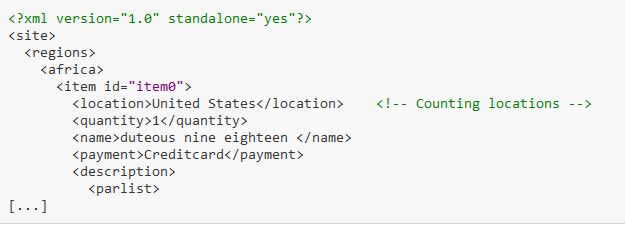
\includegraphics[width=0.75\textwidth]{figures/XML}}
	\caption{XML stream parsing dengan iterparse}
	\label{XML stream parsing dengan iterparse}
\end{figure}

